\documentclass[11pt,letterpaper]{article}
\usepackage{xcolor}
\usepackage{textcomp,marvosym}
\usepackage{amsmath,amssymb}
\usepackage[left]{lineno}
\usepackage{changepage}
\usepackage{rotating}
\usepackage{natbib}
\usepackage{setspace}
\usepackage{fancyhdr}
\usepackage{graphicx}
\usepackage{sidecap}
\usepackage{pdfpages}
\usepackage{longtable}
\usepackage{url}

\usepackage[aboveskip=1pt,labelfont=bf,labelsep=period,justification=raggedright,singlelinecheck=off]{caption}
\doublespacing

\raggedright
\textwidth = 6.5 in
\textheight = 8.25 in
\oddsidemargin = 0.0 in
\evensidemargin = 0.0 in
\topmargin = 0.0 in
\headheight = 0.0 in
\headsep = 0.5 in
\parskip = 0.1 in
\parindent = 0.2 in

\pagestyle{myheadings}
\pagestyle{fancy}
\fancyhf{}
\lhead{Swanson-Hysell et al., submitted to GEOLOGY}
\rhead{\thepage}

\begin{document}

\begin{flushleft}
{\Large \textbf{Rapid emplacement of massive Duluth Complex intrusions within the Midcontinent Rift}}
\\
Nicholas L. Swanson-Hysell\textsuperscript{1}, Steven A. Hoaglund\textsuperscript{2}, James L. Crowley\textsuperscript{3}, Mark D. Schmitz\textsuperscript{3}, Yiming Zhang\textsuperscript{1}, James D. Miller Jr.\textsuperscript{2}
\\
\bigskip
\textsuperscript{1} Department of Earth and Planetary Science, University of California, Berkeley, CA, USA\\
\textsuperscript{2} Department of Earth and Environmental Sciences, University of Minnesota, Duluth, MN, USA \\
\textsuperscript{3} Department of Geosciences, Boise State University, Boise, ID, USA
\bigskip
\end{flushleft}

\linenumbers
%\pagestyle{empty}

\section*{ABSTRACT}

The Duluth Complex is one of the largest mafic intrusive complexes in the world. It was emplaced as the Midcontinent Rift developed in Laurentia's interior during an interval of magmatism and extension from \textit{ca.} 1109 to 1084 Ma. This duration of magmatic activity is more protracted than is typical for large igneous provinces interpreted to have formed from decompression melting of upwelling mantle plumes. While the overall duration of magmatic activity was protracted, there were intervals of more voluminous magmatism. New high-precision $^{206}$Pb/$^{238}$U dates for the anorthositic and layered series of the Duluth Complex constrain these units to have been emplaced \textit{ca.} 1096 Ma in less than 1 million years. Comparison of paleomagnetic data from these units with the apparent polar wander path supports this interpretation. This timing corresponds with eruptions of the North Shore Volcanic Group. The rapid emplacement of Duluth Complex intrusions and these eruptions bear similarities to the geologically short duration of well-dated large igneous provinces. These data support hypotheses that call upon the co-location of lithospheric extension and anomalously hot upwelling mantle undergoing decompression melting. This rapid magmatic pulse occurred more than 10 million years after initial magmatic activity following more than 20$^{\circ}$$\;$of latitudinal plate motion. A likely scenario is one in which upwelling mantle encountered the base of Laurentian lithosphere and flowed via ``upside-down drainage'' to the locally thinned lithosphere of the Midcontinent Rift.

\section*{INTRODUCTION}

The Midcontinent Rift represents a protracted tectonomagmatic event in the interior of Laurentia (the North American craton). Voluminous outpouring of lava and emplacement of intrusions accompanied rift development (Fig. \ref{fig:map}). Magmatic activity initiated \textit{ca.} 1109 Ma and continued until \textit{ca.} 1084 Ma \citep{Swanson-Hysell2019a}. Preserved thicknesses of the volcanic successions range from nearly 10 km for partial sections exposed on land, such as along the North Shore of Minnesota \citep{Green2011a}, to $\sim$25 km under Lake Superior \citep{Cannon1992b}. These volcanics and associated intrusions are much more voluminous than is typical for a tectonic rifting event. Analysis of seismic data leads to an estimate that total eruptive volume exceeded 2 x 10$^6$ km$^3$ and that a much greater volume was added to the lithosphere as intrusions and an underplate \citep{Cannon1992b}. The $\sim$25 Myr duration of volcanism in the Midcontinent Rift is much longer than is typical for large igneous province emplacement associated with decompression melting of an upwelling mantle plume. Well-dated large igneous provinces, such as the Central Atlantic Magmatic Province \citep{Blackburn2013a}, the Karoo-Ferrar \citep{Burgess2015a}, and the Deccan Traps \citep{Schoene2019a, Sprain2019a} have durations of $<$1 Myr for the bulk of their magmatism. An explanation for prolonged volcanism in the Midcontinent Rift could attribute rift initiation and initial volcanism via plume arrival with continued volcanism resulting from rift-driven asthenospheric upwelling. However, the most voluminous period of magmatism occurred more than 10 million years after initial flood volcanism during an interval known as the ``main magmatic stage'' \citep{Vervoort2007a}. Main stage magmatism has been attributed to an upwelling mantle plume based both on the large volume and geochemical signatures \citep{Nicholson1990a, White1995a}.

\begin{figure}[!ht]
\noindent\includegraphics[width=0.8\textwidth]{./Figures/Duluth_Complex_map.pdf}
\centering
\caption{\small{Geologic map of NE Minnesota (simplified from \citealp{Jirsa2011a}) highlighting major intrusive complexes of the Midcontinent Rift and showing geochronology sample locations. U-Pb dates from the anorthositic and layered series of the Duluth Complex (shown in light and dark blue) indicate rapid emplacement in less than 1 million years.}}
\label{fig:map}
\end{figure}

Pioneering Midcontinent Rift geochronology utilized $^{207}$Pb/$^{206}$Pb dates on zircon from volcanics \citep{Davis1997a} and intrusions \citep{Paces1993a} to illuminate the magmatic history. Subsequent advances in U-Pb geochronology enable higher precision $^{206}$Pb/$^{238}$U dates to be used when chemical abrasion methods have mitigated Pb-loss \citep{Mattinson2005a}. An updated chronostratigraphic framework for Midcontinent Rift volcanics was recently published \citep{Swanson-Hysell2019a} that included new U-Pb dates developed using these methods (Fig. \ref{fig:dates}). With these higher precision constraints, the timing and tempo of magmatic activity within the rift can be reevaluated. Of particular interest is whether magmatic activity was continuous or punctuated by pulses. Key to evaluating this question is the timing of emplacement of intrusive rocks throughout the Midcontinent Rift, particularly the largest intrusive suite -- the Duluth Complex (Fig. \ref{fig:map}). With its arcuate area of 5630 km$^2$, the tholeiitic Duluth Complex is the second-largest exposed mafic intrusive complex on Earth \citep{Miller2002c}. It was emplaced as sheet-like intrusions into the base of a comagmatic volcanic succession with the majority of its volume associated with the anorthositic series and the layered series of gabbroic and troctolitic cumulates (\citealp{Miller2002c}; Fig. \ref{fig:map}). We present $^{206}$Pb/$^{238}$U dates from the Duluth Complex, as well as the Beaver Bay Complex, to establish the duration of Duluth Complex magmatism and contextualize it with the chronology of volcanism.

\section*{METHODS and RESULTS}

U-Pb geochronology methods for isotope dilution thermal ionization mass spectrometry (ID-TIMS) follow \citet{Schmitz2012a}. Zircon crystals were chemically abraded prior to analysis in the Boise State Isotope Geology Laboratory. Weighted means were calculated from multiple single zircon dates with some dates being excluded due to Pb-loss (Fig. \ref{fig:dates} and Table \ref{tab:geochron}).\footnote{GSA Data Repository item 2020XXX, table of individual zircon dates is available online at http://www.geosociety.org/datarepository. All paleomagnetic data and interpreted specimen directions are available to the measurement level in the MagIC database (https://earthref.org/MagIC/doi/).  All code associated with statistical tests and data visualization is available within a Zenodo repository (currently available for reviewers in this Github respository: \url{https://github.com/Swanson-Hysell-Group/2020_Duluth_Complex}).} These $^{206}$Pb/$^{238}$U dates can be compared to one another, and to the volcanic dates of \cite{Swanson-Hysell2019a}, at the level of analytical uncertainty (X error in Table \ref{tab:geochron}) given that they all have been developed using EARTHTIME tracer solutions \citep{Condon2015a}. This analytical uncertainty will be referred to when dates are reported and discussed in the text.

The Duluth Complex anorthositic series comprises plagioclase-rich gabbroic cumulates varying from anorthositic gabbro to anorthosite. Samples FC1 and FC4b are from gabbroic anorthosite exposures near the former logging town of Forest Center. A weighted mean $^{206}$Pb/$^{238}$U date for FC1 of 1095.81 $\pm$ 0.16 Ma is calculated based on 10 single zircon dates (Table \ref{tab:geochron}). The FC4b date is indistinguishable from FC1 with a weighted mean $^{206}$Pb/$^{238}$U date of 1095.71 $\pm$ 0.17 Ma based on dates from 8 zircons. These dates are indistinguishable from the weighted mean $^{206}$Pb/$^{238}$U date of 1095.86 $\pm$ 0.19 Ma developed from chemically-abraded zircons of gabbroic anorthosite sample AS3 collected from the anorthositic series in the vicinity of Duluth (\citealp{Schoene2006a}; Fig. \ref{fig:dates}, Table \ref{tab:geochron}).

% Zircon grains from these samples are commonly used as laser ablation U-Pb geochronology standards.

The layered series of the Duluth Complex is a suite of stratiform troctolitic to gabbroic cumulates that were emplaced as discrete intrusions (Fig. \ref{fig:map}). The PRI sample is a coarse-grained augite troctolite from the Partridge River intrusion which is at the base of the complex in contact with underlying Paleoproterozoic metasedimentary rocks (Fig. \ref{fig:map}). Data from 6 zircons result in a weighted mean $^{206}$Pb/$^{238}$U date of 1096.19 $\pm$ 0.19 Ma (Fig. \ref{fig:dates}). The BEI sample is a coarse-grained olivine gabbro from the Bald Eagle intrusion. This intrusion has been interpreted as one of the youngest layered series units based on cross-cutting relationships inferred from aeromagnetic data \citep{Miller2002c}. Dates from 6 zircons of BEI result in a weighted mean $^{206}$Pb/$^{238}$U date of 1095.89 $\pm$ 0.19 Ma (Fig. \ref{fig:dates}) that is indistinguishable from the anorthositic series dates.

\begin{figure}[!ht]
\noindent\includegraphics[width=\textwidth]{./Figures/MCR_Dates.pdf}
\caption{\small{Date bar plot of CA-ID-TIMS $^{206}$Pb/$^{238}$U dates for Midcontinent Rift volcanics and intrusives. Each vertical bar represents the date for an individual zircon while the horizontal lines and grey boxes represent the weighted means and their uncertainty.}}
\label{fig:dates}
\end{figure}

The Beaver Bay complex is a suite of dominantly hypabyssal intrusions that cross-cut the North Shore Volcanic Group (Fig. \ref{fig:map}). Sample HCT is an augite troctolite from the Houghtaling Creek troctolite. The medium-grained olivine-plagioclase cumulates of this intrusion are interpreted to have been emplaced as a macrodike \citep{Miller2001a}. While some zircons from HCT have Pb-loss that was not fully mitigated by chemical abrasion, dates from 4 concordant zircons result in a weighted mean $^{206}$Pb/$^{238}$U date of 1095.44 $\pm$ 0.26 Ma (Fig. \ref{fig:dates}). A sample of coarse-grained ferrodiorite was collected as WLFG from the Wilson Lake ferrogabbro of the Beaver Bay Complex. This plug-shaped zoned intrusion was emplaced into the roof zone of the Duluth Complex. Dates from 5 zircons result in a weighted mean $^{206}$Pb/$^{238}$U date of 1091.63 $\pm$ 0.35 Ma (Fig. \ref{fig:dates}). This date overlaps within uncertainty with the $^{206}$Pb/$^{238}$U date of 1091.61 $\pm$ 0.14 Ma from a Silver Bay intrusion of the Beaver Bay Complex (\citealp{Fairchild2017a}; Figs. \ref{fig:map} and \ref{fig:dates}).

\begin{table}[h!]
\footnotesize
\caption{Summary of CA-ID-TIMS $^{206}$Pb/$^{238}$U dates from Midcontinent Rift intrusions}
\begin{tabular}{|p{3 cm}|p{3 cm}|p{1.8 cm}|c|ccc|c|c|}
\hline
Sample & Group & Latitude & $^{206}$Pb/$^{238}$U & \multicolumn{3}{|c|}{Error (2$\sigma$)} & MSWD & n \\
 &  & Longitude & date (Ma) & X & Y & Z & & \\
\hline
PRI \textit{Partridge River intrusion} & Duluth Complex (layered series) & 47.5480$^{\circ}$ N 92.1074$^{\circ}$ W & 1096.19 & 0.19 & 0.36 & 1.15 & 0.45 & 6 \\
\hline
BEI \textit{Bald Eagle intrusion} & Duluth Complex (layered series) & 47.7516$^{\circ}$ N 91.5680$^{\circ}$ W & 1095.89 & 0.19 & 0.36 & 1.15 & 1.59 & 6 \\
\hline
AS3 \textit{Duluth anorthosite} & Duluth Complex (anorthositic series) & 46.7621$^{\circ}$ N 92.1590$^{\circ}$ W & 1095.86 & 0.19 & 0.36 & 1.15 & 0.43 & 8 \\
\hline
FC1 \textit{Forest Center anorthosite} & Duluth Complex (anorthositic series) & 47.7827$^{\circ}$ N 91.3266$^{\circ}$ W & 1095.81 & 0.16 & 0.34 & 1.14 & 1.44 & 10 \\
\hline
FC4b \textit{Forest Center anorthosite} & Duluth Complex (anorthositic series) & 47.7677$^{\circ}$ N 91.3753$^{\circ}$ W & 1095.71 & 0.17 & 0.35 & 1.14 & 0.38 & 8 \\
\hline
HCT \textit{Houghtaling Creek troctolite} & Beaver Bay Complex & 47.6009$^{\circ}$ N 91.1497$^{\circ}$ W & 1095.44 & 0.26 & 0.40 & 1.16 & 1.13 & 4  \\
\hline
WLFG \textit{Wilson Lake ferrogabbro} & Beaver Bay Complex & 47.6620$^{\circ}$ N 91.0619$^{\circ}$ W & 1091.63 & 0.35 & 0.46 & 1.18 & 0.74 & 5 \\
\hline
BBC-SBA1 \textit{Silver Bay aplite} & Beaver Bay Complex & 47.6620$^{\circ}$ N 91.0619$^{\circ}$ W & 1091.61 & 0.14 & 0.30 & 1.2 & 1.0 & 6 \\
\hline
\end{tabular}\\
%\begin{tablenotes}[para,flushleft]
Notes: X--internal (analytical) uncertainty in the absence of external or systematic errors; Y--uncertainty incorporating the U-Pb tracer calibration error; Z--uncertainty including X and Y, as well as $^{238}$U decay constant uncertainty (0.108$\%$; \citealp{Jaffey1971a}). This Z error needs to be utilized when comparing to dates developed using other decay systems (e.g., $^{40}$Ar/$^{39}$Ar, $^{187}$Re-$^{187}$Os); MSWD--mean square of weighted deviates; n--number of individual zircon dates included in the calculated sample mean date. All dates are from this study with the exceptions of AS3 which was published in \cite{Schoene2006a} and BBC-SBA1 which was published in \cite{Fairchild2017a}. Data for individual zircons are provided in the Data Repository.
%\end{tablenotes}
\label{tab:geochron}
\end{table}

Paleomagnetic data from sites of the layered series (37 sites) and the anorthositic series (11 sites) in the vicinity of the city of Duluth were published in \cite{Beck1970a} (Fig. \ref{fig:poles}). Statistical tests show site directions of the layered and anorthositic series to share a common mean, consistent with their overlapping U-Pb dates. In order to have paleomagnetic data directly paired with the geochronology, oriented cores were collected and analyzed from the sites of the FC1, FC4 and HCT samples. Magnetization was measured on a 2G DC-SQUID magnetometer at UC Berkeley. Samples underwent alternating field or thermal demagnetization steps and fits were made using the PmagPy software \citep{Tauxe2016a}. While \cite{Beck1970a} did not discuss or implement tilt corrections, the Duluth Complex and overlying lava flows gently dip towards Lake Superior and the paleomagnetic data need to be corrected for this tilt. We compile abundant igneous layering orientation measurements, which are similar to the orientations of overlying lavas and interflow sediments, and use them for tilt-correction.

\begin{figure}[!ht]
\noindent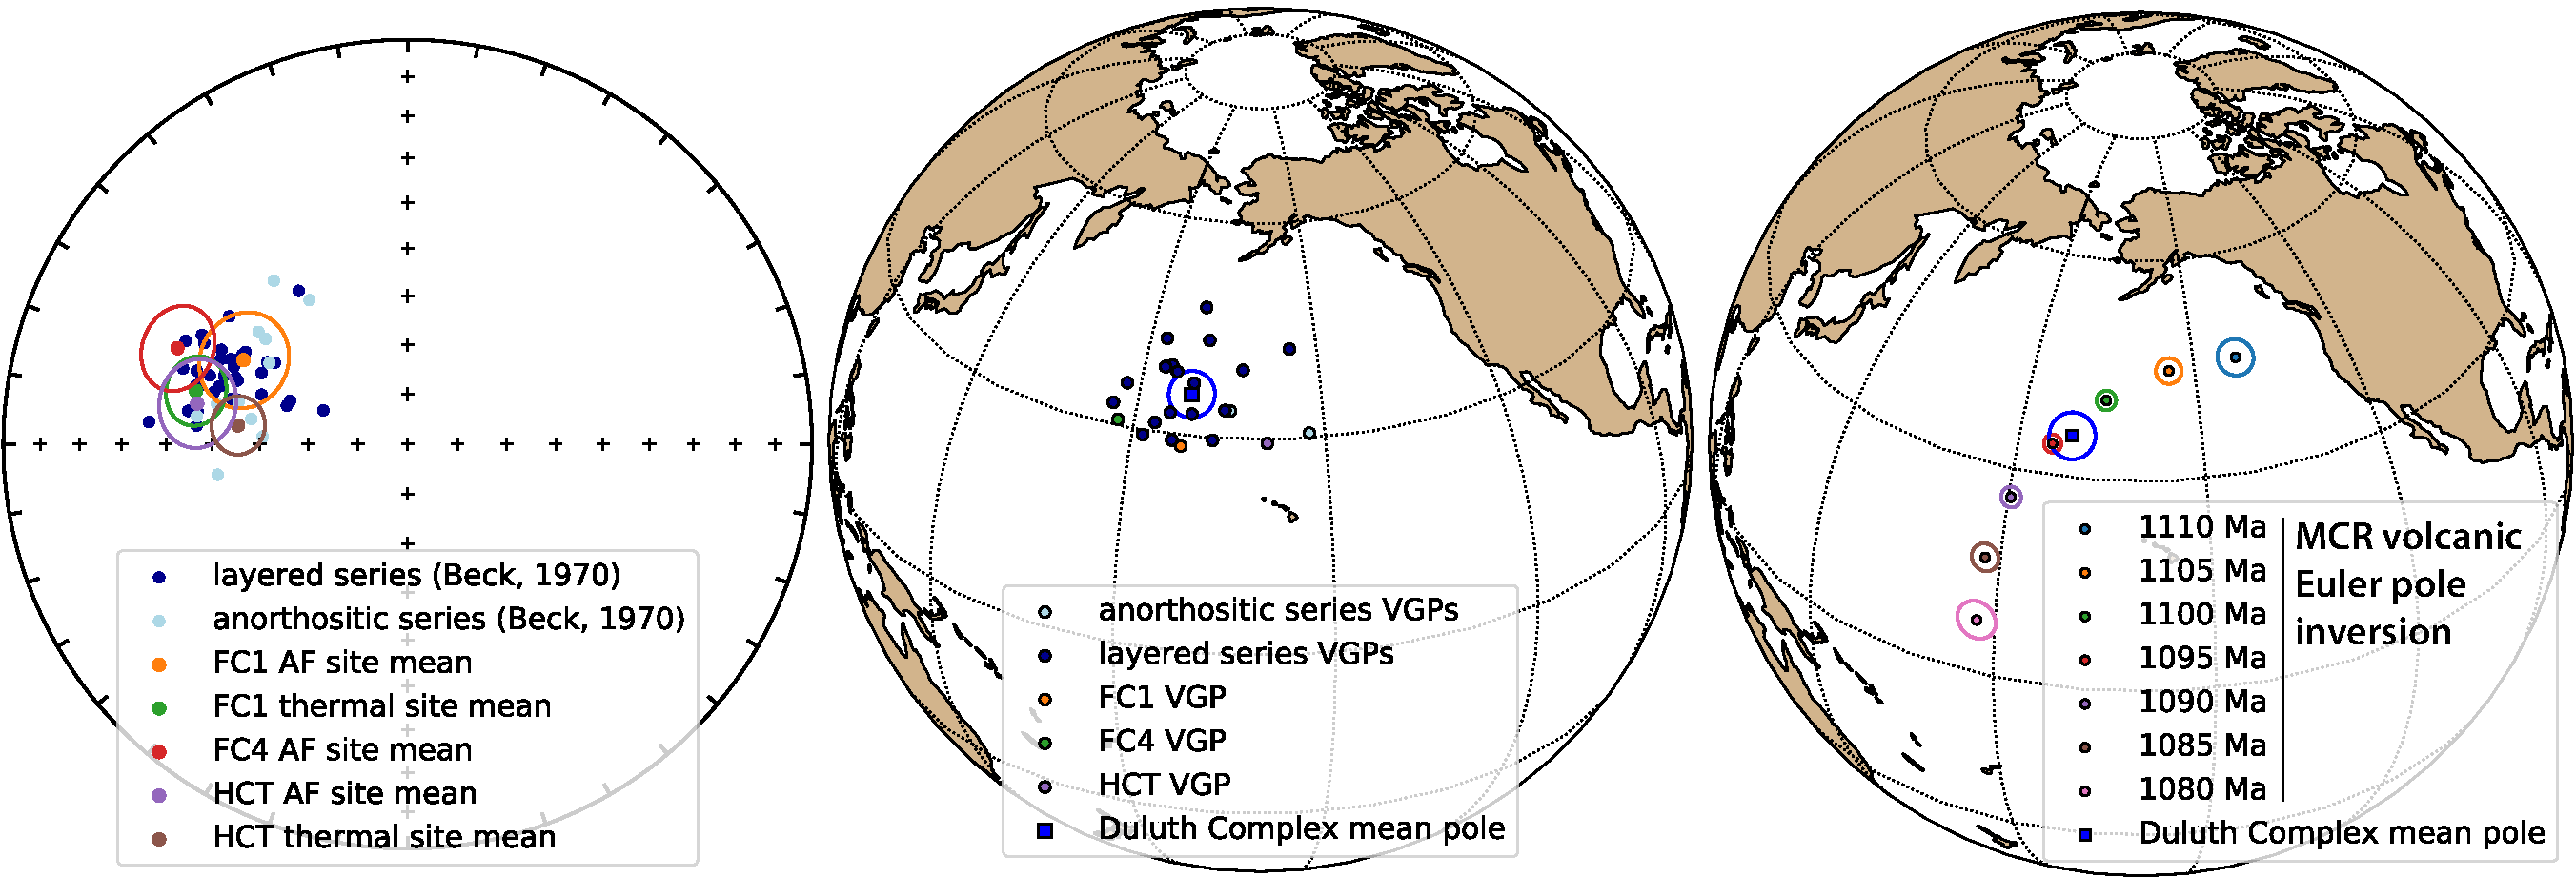
\includegraphics[width=\textwidth]{./Figures/Duluth_Complex_pole.pdf}
\caption{\small{Left panel: tilt-corrected site mean paleomagnetic directions from anorthositic and layered series sites of \cite{Beck1970a} in the vicinity of Duluth and from the FC1, FC4, and HCT sites. Center panel: Virtual geomagnetic poles (VGPs) for sites with $\alpha_{95}<15^{\circ}$ give a mean pole of: 188.7$^{\circ}$ E, 35.6$^{\circ}$ N, N=24, A$_{95}$=3.1, k=92. Right panel: Duluth Complex paleomagnetic pole shown with a synthesized pole path developed using an Euler pole inversion of Midcontinent Rift volcanic poles.}}
\label{fig:poles}
\end{figure}

The rapid progression of poles within the Midcontinent Rift apparent polar wander path (APWP) enable these paleomagnetic data to give chronological insight. The positions of poles from the early stage of rift magmatism are quite different from main stage lavas (Fig. \ref{fig:poles}). The similar position of virtual geomagnetic poles (VGPs) from across the Duluth Complex layered and anorthositic series, including the FC sites, is consistent with contemporaneous emplacement and they can be combined into a mean pole (Fig. \ref{fig:poles}). This paleomagnetic pole can be compared to a synthesized Midcontinent Rift APWP developed using an Euler pole inversion of the chronostratigraphically-constrained volcanic poles \citep{Swanson-Hysell2019a}. The Duluth Complex pole lies between the 1100 Ma and 1095 Ma path positions with the $A_{95}$ uncertainty of the pole overlapping with the two angular standard deviations ellipse of the 1095 Ma path position. This result is consistent with a \textit{ca.} 1096 Ma age for the layered and anorthositic series and strengthens the correlation with the volcanics.

%could calculate these "stage" poles at 1 Myr intervals to sharpen the pencil on this comparison

\section*{DISCUSSION}

The new U-Pb dates, together with the paleomagnetic data, imply that the bulk of both the layered series and the anorthositic series of the Duluth Complex were emplaced in less than 1 million years. With the oldest date of 1096.19 $\pm$ 0.19 Ma and the youngest of 1095.71 $\pm$ 0.17 Ma, the five dates from these series are within 500,000 years of one another and within 850,000 years if the 2$\sigma$ errors are considered (Fig. \ref{fig:dates}). This emplacement was coeval with eruption of the upper southeast sequence of the North Shore Volcanic Group (NSVG) which comprises $\sim$7900 meters of lavas and is the thickest exposed Midcontinent Rift volcanic succession. The indistinguishable ages of the anorthositic and layered series, together with coeval NSVG eruptions, indicate that \textit{ca.} 1096 Ma there was a large pulse of melt generation.

The 1095.44 $\pm$ 0.26 Ma age of the Houghtaling Creek troctolite is indistinguishable from the younger Duluth Complex dates. This result indicates that this pulse of voluminous magmatic activity is represented in some intrusions within the Beaver Bay Complex. A younger pulse of Beaver Bay Complex magmatism postdates NSVG eruptions as units such as the Beaver River diabase and the Silver Bay intrusions penetrate the youngest NSVG lavas, including the 1093.94 $\pm$ 0.28 Ma Palisade Rhyolite (\citealp{Miller2001a, Swanson-Hysell2019a}; Fig. \ref{fig:map}). The age of this magmatism is represented by the indistinguishable dates of 1091.63 $\pm$ 0.35 Ma for the Wilson Lake ferrogabbro and 1091.61 $\pm$ 0.14 Ma from the Silver Bay intrusions (Fig. \ref{fig:dates}; Table \ref{tab:geochron}). This younger Beaver Bay Complex magmatism is coeval with the eruption of the $>$5 km thick Portage Lake Volcanics that are exposed on the Keweenaw Peninsula and Isle Royale (Fig. \ref{fig:dates}).

Rapid emplacement of the voluminous layered and anorthositic series of the Duluth Complex bears similarities to the geologically short duration ($<$1 Myr) of well-dated continental flood basalt provinces \citep{Burgess2015a, Schoene2019a}. This similarity supports the hypothesis put forward by \cite{Green1983a}, and advanced by others including \cite{Cannon1992a} and \cite{Stein2015a}, that the co-location of massive magmatism and rifting is the result of lithospheric extension atop decompression melting of an upwelling mantle plume. Contemporaneous heating of Laurentia lithosphere 600 km to the north of the rift is indicated by thermochronologic data from middle to lower crustal xenoliths \citep{Edwards2018a}. Basaltic magma was also emplaced throughout the Southwest large igneous province coeval with rift magmatism, including sills more than 2300 km from Duluth \citep{Bright2014a}. That such a broad region of Laurentia lithosphere experienced heating and magmatism supports the hypothesized large-scale mantle upwelling.

%The Nd and Re-Os isotopic signatures of lava flows have been interpreted to be the result of plume-derived melts with variable interaction with continental lithospheric mantle \citep{Nicholson1997a, Shirey1997a}.

Both the \textit{ca.} 1108 early stage and \textit{ca.} 1096 Ma main stage volcanism within the Midcontinent Rift was voluminous and interpreted to be the result of a plume-related thermal anomaly. The interpretation that this volcanism is associated with a deep-seated mantle plume needs to be reconciled with the long duration of magmatism and the rapid equatorward motion of North America from a latitude of $\sim$54$^{\circ}$ N \textit{ca.} 1108 Ma during early stage flood basalt eruptions to $\sim$32$^{\circ}$ N by the \textit{ca.} 1096 Ma main stage (paleolatitudes for the location of Duluth, MN). While some of this motion could be associated with true polar wander, in which the mesosphere and asthenosphere rotated in conjunction with the lithosphere, \cite{Swanson-Hysell2019a} showed that the record of paleomagnetic poles requires a substantial component of differential plate tectonic motion. The pulsed nature of magmatic activity could support a model wherein there were multiple upwelling pulses. As postulated by \cite{Cannon1992a}, the initial pulse expressed by \textit{ca.} 1108 early stage flood basalt volcanism initiated lithospheric thinning. Given the significantly thinned lithosphere in the Midcontinent Rift region, subsequent positively-buoyant plume material that encountered Laurentia lithosphere would have experienced ``upside-down'' drainage wherein relief at the base of the lithosphere resulted in lateral and upward flow into the Midcontinent Rift \citep{Sleep1997a, Swanson-Hysell2014b}. Flow of upwelling mantle to where the lithosphere was locally thin would have led to ponding and concentrated decompression melting within the rift axis region. One scenario is that Laurentia was migrating over a plume generation zone \citep{Burke2008a} from which multiple deep-seated mantle plumes upwelled to the lithosphere over that time interval. The first could have been centered on the present-day Lake Superior region with the second encountering Laurentian lithosphere and being directed to the rift by upside-down drainage in addition to driving magmatism in southwest Laurentia. Another scenario is that \textit{ca.} 1096 Ma magmatism was invigorated by upwelling return flow enhanced by slab avalanche induced downwelling connected to the rapid plate motion of Laurentia that initiated in the early stage \citep{Swanson-Hysell2019a}. Overall, the constraint that both the anorthositic and layered series of the Duluth Complex were emplaced in less than 1 million years requires an exceptional thermal anomaly that lead to voluminous rapid melt generation during the main stage of Midcontinent Rift development.

%The indistinguishable age of rocks from the anorthositic and layered series of the Duluth Complex continue to support the model where they are genetically linked to the same episode of melt generation. The main variability between the two nearly-coeval intrusive suites comes in the concentration of plagioclase crystals with contact relationships suggesting that the crystal-ladened melts of the anorthositic complex being emplaced prior to less crystal-rich magma of the layered series intrusions \citep{Miller2002c}.

%Including a discussion of other examples of co-located massive basaltic volcanism and rifting here could be valuable: CAMP; North Atlantic; Afar

\subsection*{ACKNOWLEDGEMENTS}
Project research was supported by NSF EAR-1847277 (awarded to NLS-H) and the University of Minnesota, Duluth. Funding for the analytical infrastructure of the Boise State University Isotope Geology Laboratory was provided by NSF EAR-0824974 and EAR-0521221. Margaret Avery and Dan Costello provided field assistance. Debbie Pierce assisted with analyses at Boise State.
\footnotesize

\singlespacing

\bibliographystyle{gsabull}
\bibliography{../../../0000_Github/references/allrefs}

\newpage



%The older Felsic series and Early Gabbro series of the Duluth Complex are grouped as the ``Early series."



%The green horizontal bar represents the interval of emplacement of the layered and anorthositic series of the Duluth Complex. The orange horizontal bar represents the interval of Beaver Bay Complex magmatism represented by the Wilson Lake Ferrogabbro and the Silver Bay intrusions.



\end{document}
